\documentclass[11pt,a4paper]{article}
\usepackage[latin1]{inputenc}
\usepackage[margin=1in]{geometry}
\usepackage{amsmath}
\usepackage{amsfonts}
\usepackage{amssymb}
\usepackage{graphicx}
\usepackage{enumitem}
\usepackage{listings}
\usepackage{color}

\definecolor{dkgreen}{rgb}{0,0.6,0}
\definecolor{gray}{rgb}{0.5,0.5,0.5}
\definecolor{mauve}{rgb}{0.58,0,0.82}

\lstset{frame=tb,
 language=MatLab,
 aboveskip=3mm,
 belowskip=3mm,
 showstringspaces=false,
 columns=flexible,
 basicstyle={\small\ttfamily},
 numbers=none,
 numberstyle=\tiny\color{gray},
 keywordstyle=\color{blue},
 commentstyle=\color{dkgreen},
 stringstyle=\color{mauve},
 breaklines=true,
 breakatwhitespace=true,
 tabsize=3
}

\setlength\abovedisplayskip{0pt}
\author{James Brissette}
\title{CS-6210: HW 5}
\begin{document}
	\maketitle
	
	\section{Chapter 2}
		\begin{itemize}
			\item[2.6]
				\begin{enumerate} [label={\alph*)}]
					\item Using the bisection method, we can calculate the value of $\sqrt{\alpha}$ by looking first at the non-linear form of the function:
					\begin{align*}
						x &= \sqrt{\alpha} \\
						f(\alpha) &\equiv x^2 - \alpha = 0
					\end{align*}
					
					Using this equation we can use the bisection method to choose two points. We make sure the points we choose, $a_1$ and $b_1$, yield solutions on either side of the x-axis (e.g. $f(a)f(b) < 0$) to ensure there is a zero somewhere in between (an assumption we can only make if the function is continuous and smooth). We then take the bisection at point $c_1$ where $c_i$ is defined as $(a_i+b_i)/2$ and identify the sub interval that contains the zero (e.g. changes signs) and update our points. If it's in the left interval, $b_2$ becomes $c_1$ and $a_2 = a_1$ or else if it's in the right interval, $a_2 = c_1$ and $b_2 = c_1$.
					
					We repeat this process until our error is below our tolerance.
					
					\item Using Newton's method, we similarly solve in terms of $x$ in order to get our equation into a form in which we can differentiate it. Newton's method follows the form:
					$$x_{i+1} = x_i - \frac{f(x_i)}{f'(x_i)}$$
					Following this, we can substitute out equation into $f$ and its calculated derivative into $f'$ and calculate the next value of $x$. For example, using the function given in the problem, starting with $\alpha=36$ and $x=5$ we could iterate through and solve as follows:
					$$\begin{array}{c|c}
						x & error \\ \hline
						5 & 11 \\
						6.100000000000000e+00 & -1.209999999999994e+00 \\
						6.000819672131148e+00 & -9.836737436181409e-03 \\
						6.000000055980886e+00 &  -6.717706284575797e-07 \\
						6.000000000000001e+00 & -1.421085471520200e-14 \\
						6 & 0
					\end{array}$$
				\end{enumerate}
				See below for the MATLAB script used to generate this example:
				\begin{lstlisting}
function [output] = ch2q6(x0,alpha)
tol = 1e-16;
error = 1e10;
x = x0;
while abs(error) > tol
    f = x^2 - alpha;
    fp = 2*x;
    x = x - (f / fp);
    error = 0 - (x^2 - alpha)
end
output = x;
end
				\end{lstlisting}
			\item[2.8]
				\begin{enumerate} [label={\alph*)}]
					\item Based on the rate of convergence of the computed solution in the data table, this looks like the Newton method. We see our first iteration gives us an error of $2.5e-01$, followed by $2.5e-02$, $3.04e-04$, $4.64e-08$ and $1e-15$. Using the formula given in $2.15$, the calculated $\gamma$ here is approximately $2.66096$, $2.19537$, $2.085077$, and $2.045413$ for each respective iterative error. We know that given an initial starting point close to the solution the Newton method converges at a rate of $\gamma\approx2$ what we see here are results consistent with what we would expect from this method.
				\end{enumerate}
			\item[2.21]
				\begin{enumerate} [label={\alph*)}]
					\item Since we are given a function $f$ for which we know there must be some value $y$ such that plugging $y$ into $f$ we get zero, and we are given a function $y+x=e^{-6y}$ that is difficult to solve for $y$ in terms of $x$, we can use bisection to solve for the value of $y$ in the first equation that is necessary for us to get plugging in some value of $x$ into the second. This will allow us to find the correct value of $x$.
					
					The first step is to find the value of $y$ that gives us $f=0$, and to do this we take a starting interval for our bisection to look over. We can quickly see that in the trivial case if we plug in $0$ we get $1$ and this gives us a convenient upper bound, $b$. If we plug in $-1$ we see we get $-3$ and this is a convenient lower bound, $a$. We might also have found this by plotting the curve and estimating these bounds.
					
					We then begin bisecting the interval until we find the correct value of $y$ and we subsequently plug that into our second function to solve for the appropriate value of $x$.
					
					\item Using Newton's method is a little more challenging in that we need to solve for the first derivative. By writing $f$ as $f(y(x))$ we see that we want to solve for $f$ in terms of $x$. If we take the function $y+x=e^{-6y}$ and solve it for $y$ it gives us an equation that we then use in place of $f$ in Newton's method. Since $y$ is solved in terms of $x$ we differentiate it for the denominator and we proceed to solve.
					
					\item Using the method described in part $a$ I used the following script to solve for $y$ and then subsquently used that $y$ to solve for $x$. This gave me a value of $y=-3.221853546260856e-01$ and $x=7.233170030518265e+00$
					\begin{lstlisting}
function [output] = ch2q21()
a = -1;
b = 0;
c = (a+b)/2;

tol = 1e-16;
error = 1e10;

while abs(error) > tol
    if (a^3 + 3*a + 1)*(c^3 + 3*c + 1) < 0
        b = c;
    else
        a = c;
    end
    c = (a + b)/2;
    error = 0 - (c^3 + 3*c + 1);
end
output = c;
end
					\end{lstlisting}
				\end{enumerate}
			\item[2.22]
				\begin{enumerate} [label={\alph*)}]
					\item The second-order Taylor approximation centered at $x_i$ takes the form
					$$f(x) = f(x_i) + f'(x_i)(x-x_i) + \frac{1}{2}f''(x_i)(x-x_i)^2$$
					Using the quadratic formula to solve for $x$ we have
					\begin{align*}
						(x-x_i) &= \frac{-f'(x_i)\pm \sqrt{f'(x_i)^2-2f''(x_i)f(x_i)}}{f''(x_i)} \\
						x &= x_i - \frac{f'(x_i)\pm \sqrt{f'(x_i)^2-2f''(x_i)f(x_i)}}{f''(x_i)}
					\end{align*}
					
					\item There are a few things that seem to be potential issues. First, calculating the square root every time requires solving both the first and second derivatives which may not be feasible on complicated functions and which otherwise may be very computationally expensive. Next, the $\pm$ introduces additional logic that must be evaluated to determine which sign to use. Third, given the author's comment that this approximation may be more accurate when you are close to the solution, it begs the question whether these additional calculations will amplify your error when poor initial starting points are selected.
					
					\item Because you are close to the solution, you run into an issue where your function appears linear. This problem makes manifest in the second derivative beginning to approximate zero, however, we see that we can rearrange terms in order to alleviate this.
					\begin{align*}
						x &= x_i - \frac{f'(x_i)\pm \sqrt{f'(x_i)^2-2f''(x_i)f(x_i)}}{f''(x_i)} \\
						x &= x_i - \frac{f'(x_i)}{f''(x_i)} \pm\frac{\sqrt{f'(x_i)^2-2f''(x_i)f(x_i)}}{f''(x_i)}
					\end{align*}
					We can get rid of this issue by find a way to cancel the $f''$ terms in the denominator. We do this by factoring out the $f'^2$ term in the square root.
					\begin{align*}
						x &= x_i - \frac{f'(x_i)\pm \sqrt{f'(x_i)^2-2f''(x_i)f(x_i)}}{f''(x_i)} \\
						x &= x_i - \frac{f'(x_i)}{f''(x_i)} \pm\frac{\sqrt{f'(x_i)^2\Big(1-\frac{2f''(x_i)f(x_i)}{f'(x_i)^2}\Big)}}{f''(x_i)} \\
						x &= x_i - \frac{f'(x_i)}{f''(x_i)} \pm \frac{\vert f'(x_i)\vert}{f''(x_i)} *\frac{\sqrt{1-\frac{2f''(x_i)f(x_i)}{f'(x_i)^2}}}{f''(x_i)}
					\end{align*}
					We can approximate $\sqrt{1-x}$ as $1-\frac{1}{2}x$ using a Taylor expansion. Substituting this result into the numerator, we see:
					\begin{align*}
						x &= x_i - \frac{f'(x_i)}{f''(x_i)} \pm \frac{\vert f'(x_i)\vert}{f''(x_i)} *\frac{1-\frac{f''(x_i)f(x_i)}{f'(x_i)^2}}{f''(x_i)} \\
						x &= x_i - \frac{f'(x_i)}{f''(x_i)} \pm \frac{\vert f'(x_i)\vert}{f''(x_i)}-\frac{f(x_i)}{f'(x_i)} \\
					\end{align*}
					
					Now we can see that in order to get rid of the absolute value symbol, when $f'>0$ then the numerator is positive and we can get rid of it, no problem. If $f'<0$ then the absolute value would indicate we need to subtract subtract the negative so we still have a positive value in the numerator. Depending on what sign $f'$ takes we will want to select the sign that allows us to cancel out both terms.
					\item We know from the Newton Method that $x_{i+1} = x_i - \frac{f(x_i)}{f'(x_i)}$. By rearranging the terms we can solve for the equation given in the problem as follows:
					\begin{align*}
						x_{i+1} &= x_i - \frac{f(x_i)}{f'(x_i)} \\
						x_{i+1} - x_i &=  - \frac{f(x_i)}{f'(x_i)} \\
						(x_{i+1} - x_i)(x_{i+1} - x_i) &=  - (x_{i+1} - x_i) \frac{f(x_i)}{f'(x_i)} \\
						(x_{i+1} - x_i)^2 &=  - (x_{i+1} - x_i) \frac{f(x_i)}{f'(x_i)}
					\end{align*}
					Substituting this into our second-order Taylor approximation gives the following:
					\begin{align*}
						0 &= f(x_i) + f'(x_i)(x_{i+1}-x_i) - \frac{1}{2}f''(x_i)(x_{i+1} - x_i) \frac{f(x_i)}{f'(x_i)} \\
						0 &= f(x_i) + (x_{i+1}-x_i)\Big[f'(x_i) - \frac{1}{2}f''(x_i)\frac{f(x_i)}{f'(x_i)}\Big] \\
						x_{i+1} &= x_i - \frac{f(x_i)}{f'(x_i) - \frac{1}{2}f''(x_i)\frac{f(x_i)}{f'(x_i)}}*\frac{2f'(x_i)}{2f'(x_i)}\\
						x_{i+1} &= x_i - \frac{2f(x_i)f'(x_i)}{2f'(x_i)^2 - f''(x_i)f(x_i)}
					\end{align*}
				\end{enumerate}
			\item[2.25]
				\begin{enumerate} [label={\alph*)}]
					\item After some arithmetic, one finds that the derivative of $\frac{1-e^{-10x}}{1+e^{-10x}}$ is $\frac{20e^{10x}}{(e^{10x}+1)^2}$. Examining this expression at all values of x, we see that that for very large values (in absolute magnitude) the expression approaches 0, and that for small values of $x$ it is strictly positive. This can be seen from the below plot as well.
					\begin{center}
						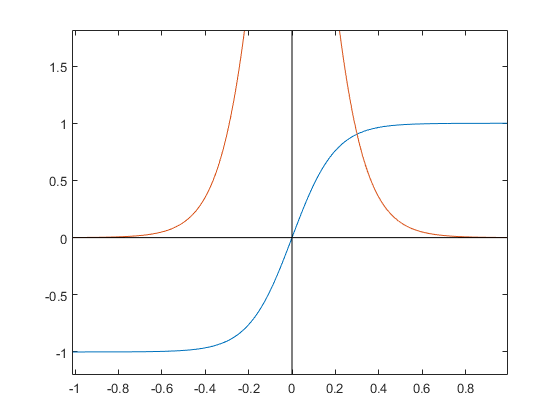
\includegraphics[width=.75\linewidth]{ch2q25c}
					\end{center}
					
					\item If we use Newton's method to solve for the next value of $x$ where $x_0=1$ we see:
					$$1 - \frac{\big(1-e^{-10}\big)\big(e^{10}+1\big)^2}{\big(1+e^{-10}\big)\big(20e^{10}\big)} = -1100.323287$$
					and we notice a similar trend with $x=-1$ and in both cases if we calculate Newton's method at each step the function diverges.
					
					\item Plugging in different values for $x_0$ I found that the method converges only when the initial starting value is lest than $0.217$ in absolute value.
					\begin{lstlisting}
function [output] = ch2q25(x0)
tol = 1e-16;
error = 1e10;
x = x0;
while abs(error) > tol
    f = (1-exp(-10*x))/(1+exp(-10*x));
    fp = 20*exp(10*x)/(exp(10*x)+1)^2;
    x = x - (f / fp);
    error = 0 - (1-exp(-10*x))/(1+exp(-10*x))
end
output = x;
end
					\end{lstlisting}
					
					\item The positive solution of $2xf'(x) = f(x)$ represents the point on the curve at which if we calculate Newton's method, we begin to oscillate back and forth without ever reaching a solution. Anything outside of that causes the method to diverge, and anything less than that would allow Newton's method to converge to the correct solution.
					
					If we were to find a point such that performing Newton's method gave us the negative value of our starting point, we would see that every subsequent iteration would continue to give us the same value and flip the sign. The calculation of that point would look like:
					\begin{align*}
						-x &= x - \frac{f(x)}{f'(x)} \\
						-2x &= -\frac{f(x)}{f'(x)} \\
						2xf'(x) &= f(x)
					\end{align*}
					That point is illustrated by the intersection of the curves.
					The graph below shows the points in question:
					\begin{center}
						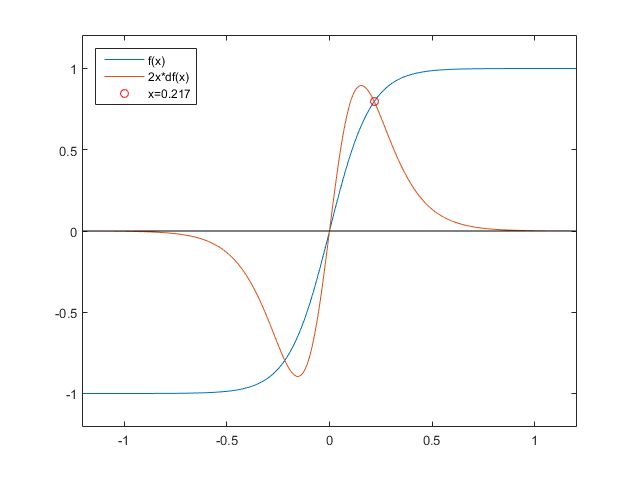
\includegraphics[width=1\linewidth]{ch2q25d}
					\end{center}
				\end{enumerate}
		\end{itemize}
		
	\section{Chapter 8}
		\begin{itemize}
			\item[8.5]
				\begin{enumerate} [label={\alph*)}]
					\item In order to solve this to find the values of $p$ and $\varepsilon$ that minimize the function, we need to solve for the partial derivatives of $E(p,\varepsilon)$:
					\begin{align*}
						E &= \sum\limits_{i=1}^n \Big[\frac{p}{1+\varepsilon cos \theta} - r_i\Big]^2 \\
						\frac{\partial E}{\partial p} &= \sum\limits_{i=1}^n 2\Big[\frac{p}{1+\varepsilon cos \theta} - r_i\Big]\Big[\frac{1}{1+\varepsilon cos \theta}\Big] = 0 \\
						\frac{\partial E}{\partial \varepsilon}&= \sum\limits_{i=1}^n 2\Big[\frac{p}{1+\varepsilon cos \theta} - r_i\Big]\Big[\frac{p cos\theta}{\big(1+\varepsilon cos \theta\big)^2}\Big] = 0
					\end{align*}
					
					\item By rewriting the model function we can substitute out our values into the form $R = V_1 + V_2cos\theta$ where $R = \frac{1}{r}$, $V_1 = \frac{1}{p}$, and $V_2 = \frac{\varepsilon}{p}$. This form allows us to treat the model function as a linear function with respect to $\theta$, but also requires us to calculate $R$ by calculating the reciprocal of $r$. $\theta$ here is not modified. Our points become $\big(\frac{1}{r},\theta\big)$.
					
					\item Solving for our new model function we find $V_1$ and $V_2$ using the partial derivatives again:
					\begin{align*}
						E(V_1,V_2) &= \sum\limits_{i=1}^n \Big[V_1 + V_2cos\theta - R_i\Big]^2 \\
						\frac{\partial E}{\partial V_1} &= \sum\limits_{i=1}^n 2\Big[V_1 + V_2cos\theta - R_i\Big] = 0\\
						\frac{\partial E}{\partial V_2} &= \sum\limits_{i=1}^n 2\Big[V_1 + V_2cos\theta - R_i\Big]\Big[cos\theta\Big] = 0
					\end{align*}
					
					Solving this as a system of equations we can set $x=A^{-1}b$ where $x=\begin{pmatrix} V_1 \\ V_2 \end{pmatrix}$, $A = \begin{pmatrix} \Sigma 1 & \Sigma cos\theta \\ \Sigma cos\theta & \Sigma cos^2\theta \end{pmatrix}$, and $z = \begin{pmatrix} \Sigma R \\ \Sigma Rcos\theta \end{pmatrix}$:
					\begin{align*}
						\begin{pmatrix} V_1 \\ V_2 \end{pmatrix} &= \frac{1}{\Sigma 1 \Sigma cos^2 \theta - \Sigma cos\theta \Sigma cos\theta} \begin{pmatrix} \Sigma cos^2 \theta & -\Sigma cos\theta \\ -\Sigma cos\theta & \Sigma 1 \end{pmatrix}\begin{pmatrix} \Sigma R \\ \Sigma Rcos\theta \end{pmatrix} \\
					\end{align*}
					If we plug each of the summations into MATLAB for computation we get:
					$$\displaystyle \sum 1 = n, \; \displaystyle \sum cos\theta = .998404, \; \displaystyle \sum cos^2\theta = 3, \; \displaystyle \sum R = 4.841513, \; \displaystyle \sum Rcos\theta = 3.162718$$
					Plugging these into our equation above, we get that
					$$\begin{pmatrix} V_1 \\ V_2 \end{pmatrix} = \begin{pmatrix} .81173398 \\ .78409506 \end{pmatrix}$$
					Using these to solve for $p$ and $\varepsilon$ we see $p = \frac{1}{V_1} = 1.231930685$ and $\varepsilon = V_2*p = .965950762$
					
					
					\item Solving using the relative least squares function we find $V_1$ and $V_2$ using the partial derivatives again:
					\begin{align*}
						E(V_1,V_2) &= \sum\limits_{i=1}^n \Big[\frac{V_1 + V_2cos\theta - R_i}{R_i}\Big]^2 \\
						\frac{\partial E}{\partial V_1} &= \sum\limits_{i=1}^n 2\Big[\frac{V_1 + V_2cos\theta - R_i}{R_i}\Big]\Big[\frac{1}{R_i}\Big] = 0\\
						\frac{\partial E}{\partial V_2} &= \sum\limits_{i=1}^n 2\Big[\frac{V_1 + V_2cos\theta - R_i}{R_i}\Big]\Big[\frac{cos\theta}{R_i}\Big] = 0
					\end{align*}
					This changes our matrix $A$ to be $\begin{pmatrix} \Sigma \frac{1}{R^2} & \Sigma \frac{cos\theta}{R^2} \\ \Sigma \frac{cos\theta}{R^2} & \Sigma \frac{cos^2\theta}{R^2} \end{pmatrix}$ where we see a common $R^2$ under each term. This then changes our calculation of $V_1$ and $V_2$ and we get:
					$$\begin{pmatrix} V_1 \\ V_2 \end{pmatrix} = \begin{pmatrix} .0026229460 \\ .1891379693 \end{pmatrix}$$
					Using these to solve for $p$ and $\varepsilon$ we see $p = \frac{1}{V_1} = 1.2429$ and $\varepsilon = V_2*p \approx .9232$
					This turns out to approximate the actual data points better than the original function and so if we had to choose, we should use this version.
				\end{enumerate}
			\item[8.6]
				\begin{enumerate} [label={\alph*)}]
					\item Starting with $y=v_1x^{v_2}$, we can re-write $y$ in terms of $x$ as $g(x)=v_1x^{v_2}$. Taking the log of both sides, we get the form given in $8.29$:
					$$G(X) = V_1 + V_2X$$
					Taking the log of the right side we see $G(X) = log(v_1) + v_2log(x)$, and accordingly we see $V_1=log(v_1)$, $X = log(X)$, and $V_2 = v_2$. From $X = log(x)$ we conclude that for any $X_i = log(x_i$ and from taking the log of the left side of the equation, $G(X) = log(g(x)) = log(y) = Y$ and so $Y_i = log(y_i)$
					
					\item We know from part a that $V_1 = logv_1$ and $V_2 = v_2$. We know further that $X = log(x)$ and $Y = log(y)$. Solving for these using the model function we can take the partial derivatives of $E$:
					\begin{align*}
						E(V_1,V_2) &= \sum\limits_{i=1}^n \Big[V_1 + V_2X_i - Y_i\Big]^2 \\
						\frac{\partial E}{\partial V_1} &= \sum\limits_{i=1}^n 2\Big[V_1 + V_2X_i - Y_i\Big] = 0\\
						\frac{\partial E}{\partial V_2} &= \sum\limits_{i=1}^n 2\Big[V_1 + V_2X_i - Y_i\Big]\Big[X_i\Big] = 0
					\end{align*}
					Then setting up our system of equations as matrices:
					\begin{align*}
						\begin{pmatrix} v_1 \\ v_2 \end{pmatrix} = \frac{1}{n\Sigma X^2 - \Sigma X \Sigma X \big)}\begin{pmatrix} 
						\Sigma X^2 & -\Sigma X \\
						-\Sigma X & N
						\end{pmatrix}\begin{pmatrix}
						\Sigma Y \\
						\Sigma YX
						\end{pmatrix}
					\end{align*}
					Solving for $V_1$ and $V_2$ and raising each to 10, we arrive back at $v_1$ and so on.
					\item If we again set up a partial derivative for $E(v_1,v_2)$ we get:
					\begin{align*}
						E(v_1,v_2) &= \sum\limits_{i=1}^n \Big[v_1x_i^{v_2}-y_i\Big]^2 \\
						\frac{\partial E}{\partial v_1} &= \sum\limits_{i=1}^n 2\Big[v_1x_i^{v_2}-y_i\Big]\Big[x_i\Big] = 0 \\
						0 &= \sum\limits_{i=1}^n \Big[v_1x_i^{v_2}-y_i\Big]\Big[x_i^{v_2}\Big] \\
						0 &= \sum\limits_{i=1}^n v_1x_i^{2v_2}-y_ix_i^{v_2} \\
						v_1\sum x_i^{2v_2} &= \sum y_ix_i^{v_2} \\
						v_1 &= \frac{\sum y_ix_i^{v_2}}{\sum x_i^{2v_2}}
					\end{align*}
					
					\item Continuing from part c, calculating the partial derivative of $E$ with respect to $v_2$ turns out to be very difficult. We reduce it to:
					\begin{align*}
						E(v_1,v_2) &= \sum\limits_{i=1}^n \Big[v_1x_i^{v_2}-y_i\Big]^2 \\
						\frac{\partial E}{\partial v_2} &= \sum\limits_{i=1}^n 2\Big[v_1x_i^{v_2}-y_i\Big]\Big[\frac{\partial}{\partial v_2}\Big] = 0 
					\end{align*}
					Seeing as how $v_2$ is currently an exponent, solving using Newton's method would require us to solve full form the derivative (which would be a messy exercise, whereas the secant method allows us a means to approximate the derivative which in our case is extremely useful. This has broader applications in that it is likely often very difficult in practice to calculate derivatives and highlights why newer machine learning libraries are beginning to feature automatic differentiation.
				\end{enumerate}
			\item[8.16]
				\begin{enumerate} [label={\alph*)}]
					\item By taking the partial derivatives of E with respect to $v_1$ and $v_2$ and setting them equal to 0 we can arrive at the equation for $\begin{pmatrix} v_1 \\ v_2 \end{pmatrix}$ as follows:
					\begin{align*}
						E(v_1,v_2) &= \sum\limits_{i=1}^n \Big[v_1p(x) + v_2q(x) - y_i\Big]^2 \\
						\frac{\partial E}{\partial v_1} &= \sum\limits_{i=1}^n 2\Big[v_1p(x) + v_2q(x) - y_i\Big]\Big[p(x)\Big] = 0 \\
						&= \displaystyle \sum v_1p^2 + \displaystyle \sum v_2 pq = \displaystyle \sum y_i p \\
						\frac{\partial E}{\partial v_2} &= \sum\limits_{i=1}^n 2\Big[v_1p(x) + v_2q(x) - y_i\Big]\Big[q(x)\Big] = 0 \\
						&= \displaystyle \sum v_1pq + \displaystyle \sum v_2 q^2 = \displaystyle \sum y_i q
					\end{align*}
					Rewriting this in matrix form to solve the similar $Ax=b$, we multiply both sides by $A^-1$ which we calculate using the formula for the inverse of a 2x2 matrix given
					\begin{align*}
						A = \begin{pmatrix} \Sigma p^2 & \Sigma pq \\ \Sigma pq & \Sigma q^2 \end{pmatrix}, \quad A^{-1} = \frac{1}{\Sigma p^2\Sigma q^2 - \big(\Sigma pq \big)^2}\begin{pmatrix} 
						\Sigma q^2 & -\Sigma pq \\
						-\Sigma pq & \Sigma p^2
						\end{pmatrix}
					\end{align*}
					we solve for $x = A^{-1}b$:
					$$\begin{pmatrix} v_1 \\ v_2 \end{pmatrix} = \frac{1}{\Sigma p^2\Sigma q^2 - \big(\Sigma pq \big)^2}\begin{pmatrix} 
						\Sigma q^2 & -\Sigma pq \\
						-\Sigma pq & \Sigma p^2
						\end{pmatrix}\begin{pmatrix}
						\Sigma py \\
						\Sigma qy
						\end{pmatrix}$$
						where $p,q,$ and $y$ are $p_i,q_i$ and $y_i$ respectively.
						
						\item If we plug in $p(x)=1$ and $q(x)=x$ into our equation above we see that the sum from 1 to $n$ of 1 is $n$, and so:
						\begin{align*}
							\begin{pmatrix} v_1 \\ v_2 \end{pmatrix} &= \frac{1}{\Sigma p^2\Sigma q^2 - \big(\Sigma pq \big)^2}\begin{pmatrix} 
						\Sigma q^2 & -\Sigma pq \\
						-\Sigma pq & \Sigma p^2
						\end{pmatrix}\begin{pmatrix}
						\Sigma py \\
						\Sigma qy
						\end{pmatrix} \\
						&= \frac{1}{n\Sigma x^2 - \big(\Sigma x \big)^2}\begin{pmatrix} 
						\Sigma x^2 & -\Sigma x \\
						-\Sigma x & n
						\end{pmatrix}\begin{pmatrix}
						\Sigma y \\
						\Sigma xy
						\end{pmatrix}
						\end{align*}
						And this is exactly the formula given in 8.12
						
						\item Plugging in $p(x) = x$ and $q(x)=x^2$ into our formula and solving using our data table we have the following:
						$$\displaystyle \sum x^2 = 2\pi^2, \; \displaystyle \sum x^3 = 0, \; \displaystyle \sum x^4 = 2\pi^4, \; \displaystyle \sum xy = \pi, \; \displaystyle \sum x^2y = 3\pi^2$$
						\begin{align*}
						\begin{pmatrix} v_1 \\ v_2 \end{pmatrix} &= \frac{1}{\Sigma x^2\Sigma x^4 - \big(\Sigma x^3 \big)^2}\begin{pmatrix} 
						\Sigma x^4 & -\Sigma x^3 \\
						-\Sigma x^3 & \Sigma x^2
						\end{pmatrix}\begin{pmatrix}
						\Sigma xy \\
						\Sigma x^2y
						\end{pmatrix}
						 \\
						&= \frac{1}{4\pi^6}\begin{pmatrix} 
						2\pi^4 & 0 \\
						0 & 2\pi^2
						\end{pmatrix}\begin{pmatrix}
						\pi \\
						 3\pi^2
						\end{pmatrix} \\
						&= \begin{pmatrix} 
						\frac{1}{2\pi^2} & 0 \\
						0 & \frac{1}{2\pi^4}
						\end{pmatrix}\begin{pmatrix}
						\pi \\
						 3\pi^2
						\end{pmatrix} \\
						\begin{pmatrix} v_1 \\ v_2 \end{pmatrix} &= \begin{pmatrix} \frac{1}{2\pi} \\ \frac{3}{2\pi^2} \end{pmatrix} 
						\end{align*}
						And here we have that $v_1 = \frac{1}{2\pi}$ and $v_2 = \frac{3}{2\pi^2}$
						
						\item This doesn't work for $p(x) = sin(x)$ and $q(x) = sin(2x)$ for the simple reason that when we evaluate $sin(x)$ at $x=\pi$ we have that $sin(\pi)=0$. This is the case for $sin(-\pi)$, $sin(0)$, and $sin(\pi)$. Because this term appears in the denominator of our determinant, we can't solve using this function.
						
						\item The solution in part a is only defined when there is linear independence between the vectors $p$ and $q$. If the angle $\theta$ between them is $0$ or $\pi$ then the vectors lie on top of each other point in either the same or opposite directions. This is akin to taking some vector $w$ and defining $p$ and $q$ in terms of a transformation of $w$ by some scaling factor, (e.g. $p = \alpha w$, $q = \beta w$) but does not imply linear independence. The vectors lie on the same line but are stretched or flipped by some factor.
						
						\item The matrix $A$ as defined in 8.16 is:
						$$ A = \begin{pmatrix}
							\phi_1(x_1) & \phi_2(x_1) \\
							\phi_1(x_2) & \phi_2(x_2) \\
							\phi_1(x_3) & \phi_2(x_3)
						\end{pmatrix} = 
						\begin{pmatrix}
							p(x_1) & q(x_1) \\
							p(x_2) & q(x_2) \\
							p(x_3) & q(x_3)
						\end{pmatrix}$$
						Saying the columns of A are independent is equivalent to saying the vectors $p$ and $q$ are linearly independent. Additionally , without independence it is not necessarily possible to prove positive definiteness of $A^TA$ and so we are unable to use the several methods derived in the text book (as linear independence has been a hallmark of our assumptions this semester).
						
						\item For part d, $p(x)$ was $sin(x)$ and $q(x)$ was $sin(2x)$. Represented at vectors, we have $p = (0,0,0)$ and $q = (0,0,0)$ as sin of any multiple of $\pi$ or 0 is 0.
						
						\item Given what we concluded in parts e and f, part a would not be defined if $q=(1,-1,1)$ or if $q=(-1,1,-1)$. Otherwise we would have:
						$$\frac{1}{\Sigma p^2\Sigma q^2 - \big(\Sigma pq \big)^2} = \frac{1}{9 - \big(3 \big)^2} = \frac{1}{0}$$
						and
						$$\frac{1}{\Sigma p^2\Sigma q^2 - \big(\Sigma pq \big)^2} = \frac{1}{9 - \big(-3 \big)^2} = \frac{1}{0}$$
				\end{enumerate}
		\end{itemize}	
\end{document}